\section{Electric Flux and Path Summations}

\underline{\textbf{Part 1}} \par
Recall from class that when a point charge is located at the corner of a cube the electric flux through one of the opposite sides is $q / 24 \epsilon_0$.
Confirm this result (approximately) with the following procedure:

\begin{enumerate}
\item Divide the side of the cube into a 3x3 grid (as shown)
\item Calculate the electric field at the center of each grid square
\item Take the dot product of each of the 9 calculated electric fields with that grid square's area vector
\item Sum the 9 results above
\item Repeat with a 4x4 grid to show that more grid squares gives a better approximation to the exact result
\end{enumerate}

\begin{figure}[H]
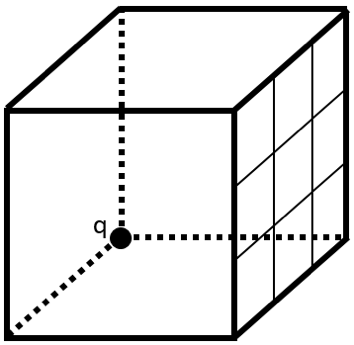
\includegraphics[scale=1.0]{figures/electric-flux-and-path-integral/fig1.png}
\end{figure}

\underline{\textbf{Part 2}} \par

See the figure below.
Calculate the change in electric potential between points A $(0, 1)$ and B $(2, 1)$ along the three paths shown.
Show all work!
Note that the two parts of path (1) are parallel and perpendicular to the electric field.
Extra credit (5\%): repeat for the path defined by the parabola $y = 2x^2 - 4x + 1$.

\begin{figure}[H]
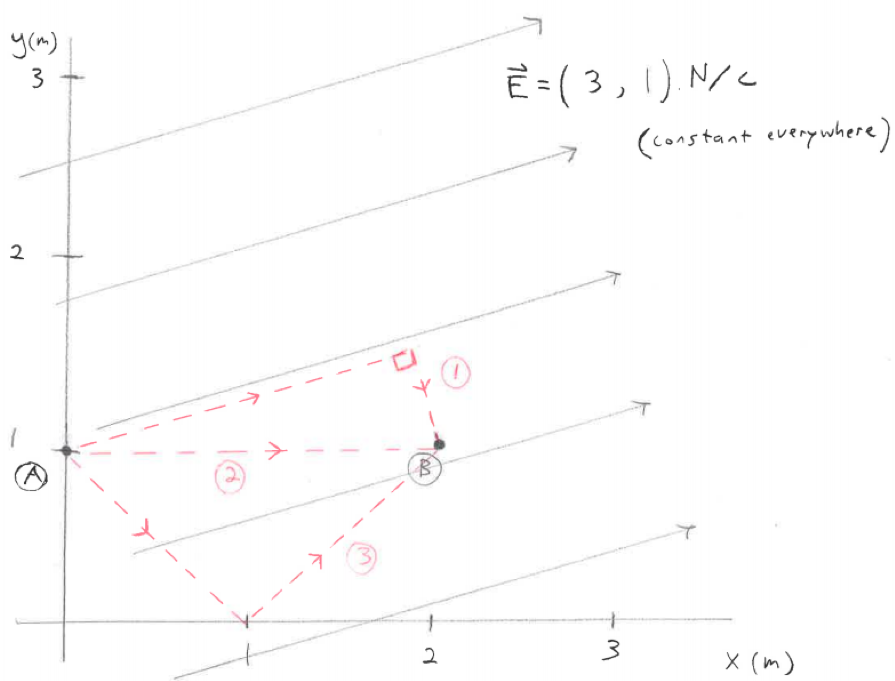
\includegraphics[scale=1.0]{figures/electric-flux-and-path-integral/fig2.png}
\end{figure}

\pagebreak \clearpage
